\chapter{Examenes de teoría}
\section{Examen mayo 2020}

\qs{Ejercicio 1 (1.5 puntos)}{
    En el almacén de una fábrica se tienen varios reactores que ya no se utilizan. El departamento de Desarrollo quiere emplearlos para estudiar nuevos procesos de producción. A cada uno de ellos le realiza estudios del grado de mezcla mediante experimentos estímulo-respuesta en impulso. Obtiene los siguientes datos:

    \textbf{Reactor 1:}
    \begin{center}
        \begin{tabular}{|c|c|c|c|c|c|}
            \hline
            $\theta$     & 0 & 0.5 & 1.0      & 1.5 & 2.0 \\ \hline
            $C_B/C_{BR}$ & 0 & 0   & $\infty$ & 0   & 0   \\ \hline
        \end{tabular}
    \end{center}

    \textbf{Reactor 2:}
    \begin{center}
        \begin{tabular}{|c|c|c|c|c|c|c|c|c|}
            \hline
            $\theta$     & 0 & 0.5  & 1.0  & 1.5  & 2.0 & 2.5  & 3.0  & 3.5 \\ \hline
            $C_B/C_{BR}$ & 0 & 0.95 & 0.45 & 0.35 & 0.2 & 0.05 & 0.02 & 0   \\ \hline
        \end{tabular}
    \end{center}

    \textbf{Reactor 3:}
    \begin{center}
        \begin{tabular}{|c|c|c|c|c|c|c|c|}
            \hline
            $\theta$     & 0 & 0.5  & 1.0  & 1.5 & 2.0  & 2.5 & 3.0 \\ \hline
            $C_B/C_{BR}$ & 0 & 0.58 & 0.37 & 0.3 & 0.15 & 0.1 & 0   \\ \hline
        \end{tabular}
    \end{center}

    \textbf{Reactor 4:}
    \begin{center}
        \begin{tabular}{|c|c|c|c|c|c|}
            \hline
            $\theta$     & 0 & 0.5 & 1.0 & 1.5 & 2.0 \\ \hline
            $C_B/C_{BR}$ & 0 & 0.6 & 0.8 & 0.6 & 0   \\ \hline
        \end{tabular}
    \end{center}

    \textbf{Reactor 5:}
    \begin{center}
        \begin{tabular}{|c|c|c|c|c|c|c|c|c|c|c|}
            \hline
            $\theta$     & 0 & 0.25  & 0.5   & 1.0   & 1.5   & 1.75  & 2.0   & 3    & 5     & 8 \\ \hline
            $C_B/C_{BR}$ & 1 & 0.779 & 0.607 & 0.368 & 0.223 & 0.174 & 0.135 & 0.05 & 0.007 & 0 \\ \hline
        \end{tabular}
    \end{center}

    De acuerdo con estos datos, para cada reactor, justifica:
    \begin{enumerate}[label={\alph*)}]
        \item el tipo de reactor
        \item la modelización más adecuada, con cálculo de parámetros si es necesario
    \end{enumerate}
}
\newpage
\solve{}
\begin{enumerate}
    \item \textbf{Reactor 1:}
          \begin{enumerate}[label={\alph*)}]
              \item Este primer reactor es un reactor tubular con un comportamiento ideal, es decir, tiene un comportamiento de flujo pistón, debido a que al graficar $E$ respecto a $\theta$, cuando el tiempo de residencia es 1 sale todo. También se puede demostrar mediante la siguiente gráfica:

                    \begin{figure}[htbp]
                        \centering
                        % Parte superior: Ecuaciones y condiciones para E
                        \begin{minipage}{0.4\textwidth}
                            \begin{align*}
                                 & \text{Para } t = t_R \text{ ó } \theta = 1 \implies E = \infty  \\
                                 & \text{Para } t \neq t_R \text{ ó } \theta \neq 1 \implies E = 0
                            \end{align*}
                        \end{minipage}
                        \hfill
                        % Parte derecha: Representación gráfica (Función Impulso y Dispersión)
                        \begin{minipage}{0.55\textwidth}
                            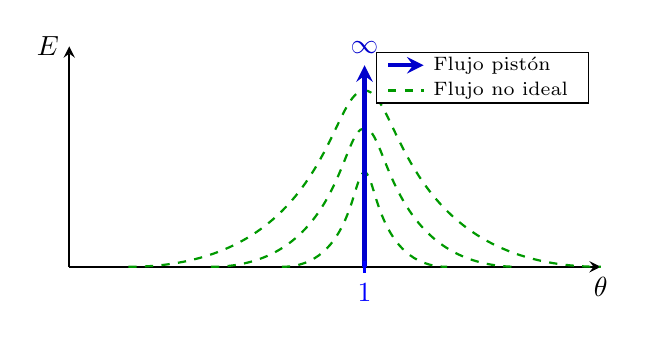
\begin{tikzpicture}[xscale=1.5, yscale=0.8]
                                % Ejes
                                \draw[->, thick] (0,0) -- (4.5,0) node[below] {$\theta$};
                                \draw[->, thick] (0,0) -- (0,3.5) node[left] {$E$};

                                % Curvas de dispersión (Campanas de Gauss - Líneas verdes discontinuas)
                                % Representan el flujo real alejándose de la idealidad
                                \draw[green!60!black, thick, dashed] (0.5,0) .. controls (2.2,0) and (2.2,2.8) .. (2.5,2.8) .. controls (2.8,2.8) and (2.8,0) .. (4.5,0);
                                \draw[green!60!black, thick, dashed] (1.2,0) .. controls (2.3,0) and (2.3,2.2) .. (2.5,2.2) .. controls (2.7,2.2) and (2.7,0) .. (3.8,0);
                                \draw[green!60!black, thick, dashed] (1.8,0) .. controls (2.4,0) and (2.4,1.5) .. (2.5,1.5) .. controls (2.6,1.5) and (2.6,0) .. (3.2,0);

                                % Función Impulso ideal (Delta de Dirac - Flujo Pistón)
                                \draw[ultra thick, blue!80!black, ->] (2.5,0) -- (2.5,3.2) node[above] {$\infty$};

                                % Etiqueta del 1 en el eje theta
                                \draw[blue, thick] (2.5,0.1) -- (2.5,-0.1) node[below] {$1$};

                                % Leyenda manual
                                \draw[fill=white, draw=black, thin] (2.6, 3.4) rectangle (4.4, 2.6);
                                \draw[ultra thick, blue!80!black, ->] (2.7, 3.2) -- (3.0, 3.2);
                                \node[right, font=\scriptsize] at (3.0, 3.2) {Flujo pistón};
                                \draw[green!60!black, thick, dashed] (2.7, 2.8) -- (3.0, 2.8);
                                \node[right, font=\scriptsize] at (3.0, 2.8) {Flujo no ideal};
                            \end{tikzpicture}
                        \end{minipage}

                        \caption{Representación de E vs $\theta$ para un reactor tubular}
                        \label{fig:sol_2020_1}
                    \end{figure}
              \item Para un reactor tubular que se comporta de una forma ideal, obviamente se va a modelizar como un reactor continuo de flujo pistón y en régimen isotermo:
                    \begin{align*}
                        \frac{d_{NA}}{dz} = n_A - (n_A +dn_A) - r_A dV                 \\
                        -dn_A = r_A dV  \leftrightarrow n_A = n_{AR}(1-x_A)            \\
                        dn_A = -n_{AR}dx_A                                             \\
                        n_{AR} \cdot dx_A = r_A dV                                     \\
                        \int_0^{V} dV = \int_{x_{A0}}^{x_{AS}} \frac{n_{AR}}{r_A} dx_A \\
                        V = n_{AR}\int_{x_{A0}}^{x_{AS}} \frac{dx_A}{r_A}              \\
                        \tau = C_{AR}\int_{x_{A0}}^{x_{AS}} \frac{dx_A}{r_A}
                    \end{align*}
                    Ademas puntualizando para varias reacciones:
                    \begin{align*}
                        -dn_i        & = r_i dV                               \\
                        F \cdot dC_i & = r_i \cdot dV = -r_i \cdot S \cdot dz \\[1ex]
                        \left.
                        \begin{aligned}
                            \frac{dC_i}{dz} & = -r_i - \frac{S}{F} \\[1ex]
                            \frac{dC_i}{dz} & = \frac{-r_i}{V}
                        \end{aligned}
                        \right\}     & \Longrightarrow \frac{F}{S} = V
                    \end{align*}
          \end{enumerate}
          \newpage
    \item \textbf{Reactor 2:}
          \begin{enumerate}[label={\alph*)}]
              \item Para discutir el tipo de reactor en este caso es necesario hacer los siguientes calculos:
                    \begin{center}
                        \begin{tabular}{|c|c|c|c|c|c|c|}
                            \hline
                            $\theta$                     & $C_B/C_{BR}$          & $\theta \cdot E$ & $\theta^2 \cdot E$    & $\int E \, d\theta$ & $\int \theta \cdot E \, d\theta$ & $\int \theta^2 \cdot E \, d\theta$ \\ \hline
                            0                            & 0                     & 0                & 0                     & 0                   & 0                                & 0                                  \\ \hline
                            0,5                          & 0,95                  & 0,475            & 0,2375                & 0,2375              & 0,11875                          & 0,059375                           \\ \hline
                            1                            & 0,45                  & 0,45             & 0,45                  & 0,35                & 0,35                             & 0,23125                            \\ \hline
                            1,5                          & 0,35                  & 0,525            & 0,7875                & 0,2                 & 0,59375                          & 0,540625                           \\ \hline
                            2                            & 0,2                   & 0,4              & 0,8                   & 0,1375              & 0,825                            & 0,9375                             \\ \hline
                            2,5                          & 0,05                  & 0,125            & 0,3125                & 0,0625              & 0,95625                          & 1,215625                           \\ \hline
                            3                            & 0,02                  & 0,06             & 0,18                  & 0,0175              & 1,0025                           & 1,33875                            \\ \hline
                            3,5                          & 0                     & 0                & 0                     & 0,005               & 1,0175                           & 1,38375                            \\ \hline
                            \multicolumn{1}{|c|}{$\sum$} & \multicolumn{3}{c|}{} & 1,01             & \multicolumn{2}{c|}{}                                                                                               \\ \hline
                        \end{tabular}
                    \end{center}
                    Donde lo fundamental es que $\int E d\theta = 1$, $\int \theta E d\theta = 1$ y $\int \theta^2 E d\theta = 1.38$.

              \item Se trata de un reactor tubular. Existen dos posibilidades para su modelización: el modelo de dispersión axial o el modelo de tanques en serie. Ambos son válidos, aunque el modelo de dispersión, basado en la ley de Fick, contempla un transporte másico (dispersión) superpuesto al flujo principal. Por tanto, es más indicado cuando la difusividad es pequeña (condiciones cercanas a la idealidad del flujo pistón). El perfil de concentraciones se caracteriza mediante el módulo de dispersión $N_D = \frac{D}{v\cdot L}$ o su inversa, el número de Péclet ($Pe = \frac{v\cdot L}{D}$).
                    Si el número de Péclet en el reactor es igual a 0, el perfil de concentración es aplanado (mezcla completa); y si tiende a infinito, corresponde a flujo pistón. Modelizando como una batería de tanques agitados en serie:
                    \begin{align*}
                        \sigma^2 & = \frac{1}{n} \implies n = \frac{1}{0.38} \approx 2.63 \implies n = 3                                                                        \\
                        \tau_i   & = \frac{\tau}{n} = \frac{\tau}{3} \cdot k = \frac{X_{A1}-X_{A0}}{1-X_{A1}} = \frac{X_{A2}-X_{A1}}{1-X_{A2}} = \frac{X_{A3}-X_{A2}}{1-X_{A3}}
                    \end{align*}
          \end{enumerate}
    \item \textbf{Reactor 3:}
          \begin{enumerate}[label={\alph*)}]
              \item Para determinar el tipo de reactor, es necesario realizar los siguientes cálculos a partir de los datos experimentales. Se ha añadido también la columna para $\theta^2 \cdot E$ y su integral, necesaria para calcular la varianza:

                    \begin{center}
                        \begin{tabular}{|c|c|c|c|c|c|c|}
                            \hline
                            $\theta$ & $C_B/C_{BR}$ & $\theta \cdot E$ & $\theta^2 \cdot E$ & $\int E \, d\theta$ & $\int \theta \cdot E \, d\theta$ & $\int \theta^2 \cdot E \, d\theta$ \\ \hline
                            0        & 0            & 0                & 0                  & 0                   & 0                                & -                                  \\ \hline
                            0,5      & 0,58         & 0,29             & 0,145              & 0,145               & 0,0725                           & -                                  \\ \hline
                            1        & 0,37         & 0,37             & 0,37               & 0,3825              & 0,2375                           & -                                  \\ \hline
                            1,5      & 0,3          & 0,45             & 0,675              & 0,55                & 0,4425                           & -                                  \\ \hline
                            2        & 0,15         & 0,3              & 0,6                & 0,6625              & 0,63                             & -                                  \\ \hline
                            2,5      & 0,1          & 0,25             & 0,625              & 0,725               & 0,7675                           & -                                  \\ \hline
                            3        & 0            & 0                & 0                  & 0,75                & 0,83                             & -                                  \\ \hline
                        \end{tabular}
                    \end{center}
                    Como se observa en la tabla, el área bajo la curva $\int E \, d\theta = 0,75 \neq 1$, por lo que forzosamente es un reactor no ideal donde se aplica el modelo de flujos mezclados; en este caso particular, la última integral (varianza) no es necesaria.
              \item Modelos mezclados: la fracción de \textit{bypass} que presenta se calcula como $1-\int E \, d\theta = 1-0,75=0,25$ y el volumen de zonas muertas (estanco) se estima como $1-\int \theta \cdot E \, d\theta = 1-0,83=0,17$. Aunque no podemos hacer los cálculos completos al no disponer de todos los datos cinéticos, la ecuación de diseño básica de un tanque agitado es la siguiente:
                    \begin{equation}
                        \tau = \frac{C_{A0}\cdot X_{AR}}{k\cdot C_{A0}(1-X_{AR})}
                    \end{equation}
          \end{enumerate}
          \newpage
    \item \textbf{Reactor 4:}
          \begin{enumerate}[label={\alph*)}]
              \item Para caracterizar el comportamiento de este reactor, en primer lugar vamos a calcular las integrales a partir de la tabla de datos disponibles:
                    \begin{center}
                        \begin{tabular}{|c|c|c|c|c|c|c|}
                            \hline
                            $\theta$ & $C_B/C_{BR}$ & $\theta \cdot E$ & $\theta^2 \cdot E$ & $\int E \, d\theta$ & $\int \theta \cdot E \, d\theta$ & $\int \theta^2 \cdot E \, d\theta$ \\ \hline
                            0        & 0            & 0                & 0                  & 0                   & 0                                & 0                                  \\ \hline
                            0,5      & 0,6          & 0,3              & 0,15               & 0,15                & 0,075                            & 0,0375                             \\ \hline
                            1        & 0,8          & 0,8              & 0,8                & 0,5                 & 0,35                             & 0,275                              \\ \hline
                            1,5      & 0,6          & 0,9              & 1,35               & 0,85                & 0,775                            & 0,8125                             \\ \hline
                            2        & 0            & 0                & 0                  & 1                   & 1                                & 1,15                               \\ \hline
                        \end{tabular}
                    \end{center}
                    Como se observa en la tabla, el área bajo la curva es $\int E \, d\theta = 1$, por lo que la curva está perfectamente normalizada. Asimismo, $\int \theta \cdot E \, d\theta = 1$, lo que nos confirma la consistencia de los datos experimentales con el tiempo espacial del sistema. A partir de aquí, podríamos calcular la varianza como $\sigma^2 = \overline{\theta^2} - \bar{\theta}^2 = 1,15 - 1^2 = 0,15$, lo cual nos indicaría un comportamiento intermedio y podríamos modelizarlo mediante tanques en serie o dispersión axial.
          \end{enumerate}

    \item \textbf{Reactor 5:}
          \begin{enumerate}[label={\alph*)}]
              \item Al igual que en los reactores anteriores, procedemos a integrar numéricamente los datos experimentales para obtener los momentos de la distribución de tiempos de residencia (RTD):
                    \begin{center}
                        \begin{tabular}{|c|c|c|c|c|c|c|}
                            \hline
                            $\theta$ & $C_B/C_{BR}$ & $\theta \cdot E$ & $\theta^2 \cdot E$ & $\int E \, d\theta$ & $\int \theta \cdot E \, d\theta$ & $\int \theta^2 \cdot E \, d\theta$ \\ \hline
                            0        & 1            & 0                & 0                  & 0                   & 0                                & 0                                  \\ \hline
                            0,25     & 0,779        & 0,19475          & 0,0487             & 0,22238             & 0,024                            & 0,006                              \\ \hline
                            0,5      & 0,607        & 0,3035           & 0,15175            & 0,39563             & 0,087                            & 0,031                              \\ \hline
                            1        & 0,368        & 0,368            & 0,368              & 0,63938             & 0,255                            & 0,161                              \\ \hline
                            1,5      & 0,223        & 0,3345           & 0,50175            & 0,78713             & 0,430                            & 0,379                              \\ \hline
                            1,75     & 0,174        & 0,3045           & 0,5329             & 0,83675             & 0,510                            & 0,508                              \\ \hline
                            2        & 0,135        & 0,27             & 0,54               & 0,8754              & 0,582                            & 0,642                              \\ \hline
                            3        & 0,05         & 0,15             & 0,45               & 0,96788             & 0,792                            & 1,137                              \\ \hline
                            5        & 0,007        & 0,035            & 0,175              & 1,02                & 0,977                            & 1,762                              \\ \hline
                            8        & 0            & 0                & 0                  & 1,03                & 1,029                            & 2,024                              \\ \hline
                        \end{tabular}
                    \end{center}
                    Con estos datos se extrae que las integrales $\int E \, d\theta$ y $\int \theta \cdot E \, d\theta$ son aproximadamente 1 ya que podemos asumir un error de hasta el 5\% en la medida experimental, sin embargo la integral $\int \theta^2 \cdot E \, d\theta = 2,024$ es decir que $\sigma^2 = 2.024-1 \approx 1$. debido a ello tenemos un reactor tipo tanque agitado
              \item Ademas ese valor de $\sigma^2$ nos indica que estamos ante un comportamiento ideal, es decir tenemos un reactor tipo tanque agitado con comportamiento de reactor continuo mezcla perfecta.
                    \begin{equation}
                        \tau = \frac{C_{A0} X_{AR}}{k C_{A0} (1-X_{AR})}
                    \end{equation}
          \end{enumerate}
\end{enumerate}
\nt{Aunque en ningún caso se ha modelado con flujo segregado al ser una cinética de primer orden, se podria utilizar este modelo en todos los casos.}
\newpage
\qs{Ejercicio 2 (1.5 puntos)}{
    Entre los reactores anteriores (R1 - R2 - R3 - R4 - R5), justifica el reactor que elegirías para llevar a cabo los siguientes procesos de reacción. Considera como objetivo minimizar el volumen de reacción o maximizar la selectividad del proceso.

    Debes justificar también el modo de operación respecto al intercambio de materia (continuo -- discontinuo -- semicontinuo), energía (isotermo -- adiabático -- no isotermo, no adiabático) y condiciones de temperatura entre el rango $T_{\text{min}}$ -- $T_{\text{max}}$.

    Modeliza el funcionamiento del reactor en cada caso

    \begin{enumerate}[label={\alph*)}]
        \item $A + 2B \rightarrow P$ ($P$ es el producto deseado) \quad $E_{a1} > E_{a2}$ \\
              $2A + B \rightarrow Q$ (reacción secundaria)
        \item $A \rightleftharpoons B$, proceso exotérmico
        \item $A + 2B \rightarrow P$ ($P$ es el producto deseado) \quad $E_{a1} < E_{a2}$ \\
              $A + B \rightarrow Q$ (reacción secundaria)
    \end{enumerate}
}
\solve{}
\begin{enumerate}[label={\alph*)}]
    \item En primer lugar procederemos a calcular la selectividad de la reacción para elegir el selector mas adecuado.
          \label{2A_2020}
          \begin{align*}
              A +2B \xrightarrow{k_1} P \quad  & r_p = k_1 C_A C_B^2 \\
              2A + B \xrightarrow{k_2} Q \quad & r_q = k_2 C_A^2 C_B
          \end{align*}
          \begin{equation*}
              s = \frac{r1}{r1+r2} = \frac{1}{1+\dfrac{r2}{r1}}= \frac{1}{1+\dfrac{k_2\cdot C_A^2\cdot C_B}{k_1\cdot C_A \cdot C_B^2}}
          \end{equation*}
          aplicando arrehenius a la constante de velocidad y simplifcando:
          \begin{equation}
              s = \frac{1}{1+\dfrac{k_{20}}{k_{10}} \dfrac{C_A}{C_B}\cdot \text{exp}\left(\dfrac{E_{a1}-E_{a2}}{RT}\right)}
          \end{equation}
          luego para maximizar la selectividad necesitamos que $C_A$ sea lo menor posible y que $C_B$ sea lo mayor posible.\\
          Dicho esto, en esta situación siempre sera necesario un reactor tanque agitado, en configuración semicontinua, donde B estara en el tanque cargado, y A se ira añadiendo poco a poco.
          Para la temperatura como $E_{a1} > E_{a2}$ entonces $\frac{E_{a1}-E_{a2}}{RT}$ será positivo, y por tanto la temperatura deberia ser lo mas grande posible, para minimizar la exponencial y asi aumentar la selectividad.\\
          \begin{center}
              \Res{\text{Tanque agitado, semicontinuo con carga de B y alimentacion suave de A, a temperatura máxima posible y por lo tanto el reactor a elegir sería el R5.}}
          \end{center}
          \newpage
          \begin{multicols}{2}
              \begin{equation*}
                  \left\{
                  \begin{aligned}
                      \frac{dV}{dt}   & = F                      \\[6pt]
                      \frac{dN_A}{dt} & = F \cdot C_{A0} - r_A V \\[6pt]
                      \frac{dN_B}{dt} & = - r_B V                \\[6pt]
                      \frac{dN_P}{dt} & = r_P V                  \\[6pt]
                      \frac{dN_Q}{dt} & = r_Q \cdot V
                  \end{aligned}
                  \right.
              \end{equation*}

              \begin{equation*}
                  \left\{
                  \begin{aligned}
                      \frac{dC_A}{dt} & = \frac{F}{V}\cdot (C_{A0}-C_A) - r_A \\[6pt]
                      \frac{dC_B}{dt} & = -\frac{F C_B}{V} - r_B              \\[6pt]
                      \frac{dC_P}{dt} & = -\frac{F C_P}{V} + r_P              \\[6pt]
                      \frac{dC_Q}{dt} & = -\frac{F C_Q}{V} + r_Q
                  \end{aligned}
                  \right.
              \end{equation*}

              \columnbreak

              \begin{equation*}
                  \left\{
                  \begin{aligned}
                      C_A             & = \frac{N_A}{V}                                \\[6pt]
                      C_B             & = \frac{N_B}{V}                                \\[6pt]
                      C_P             & = \frac{N_P}{V}                                \\[6pt]
                      C_Q             & = \frac{N_Q}{V}                                \\[6pt]
                      dN_i            & = d(V \cdot C_i) = V \cdot dC_i + C_i \cdot dV \\[6pt]
                      \frac{dN_i}{dt} & = V \cdot \frac{dC_i}{dt} + C_i \frac{dV}{dt}  \\[6pt]
                      \frac{dV}{dt}   & = F
                  \end{aligned}
                  \right.
              \end{equation*}
          \end{multicols}
    \item Para la reacción $A \leftrightarrow B$, \textbf{exotérmica}, claramente es necesario un reactor que funcione con perfil de concentraciones(o bien reactor tipo tanque discontinuo si es ideal RDMP o bien un reactor tubular en el caso de ser ideal RCFP), los reactores continuos se suelen usar para grandes producciones, ademas de que un reactor tubular es mejor para reactivos gaseosos,
          ya que se impulsa por la presión, y ademas no es necesario un agitador que requiere energia electrica, sin embargo el reactor tanque agitado es mucho mas sencillo de diseñar, y funciona muy bien para una conversión muy alta, suponiendo que tenemos mezclas liquidas la elección seria un reactor discontinuo con una progresión optima de temperatura:\\
          \textbf{Balances Reactor discontinuo}
          \begin{align*}
              \frac{dN_A}{dt}            & = r_A V \leftarrow  X_A = \frac{N_{AR}-N_A}{N_{A}}                    \\[6pt]
              NA                         & = N_{AR}(1-X_A) \leftarrow dN_A = -N_{AR}\cdot dX_A                   \\[6pt]
              dN_A \cdot \frac{dX_A}{dt} & = r_A V \implies \int_0^{t_R} dt = \int_0^{X_{Af}} \frac{dN_A}{r_A V} \\[6pt]
              t_R                        & = C_{AR}\int_0^{X_{Af}} \frac{dX_A}{r_A}
          \end{align*}
          en una reaccion irreversible siempre se puede trabajar a $T_\text{max}$ pero en las irreversibles no ($E_d < E_i$), por lo que debido a ello es necesario una temperatura baja para tener una conversión alta, pero por criterios econocomicos no es viable y debido a ello se hace una
          progresión optima de la temperatura.
          \begin{equation*}
              \frac{dr_A}{dz} = 0
          \end{equation*}
          \begin{equation*}
              0 = Ad \cdot \frac{E_d}{RT^2} \cdot \text{exp}\left(\frac{-E_d}{RT}\right) - C_{A0} \cdot (1-X_A) - A_i \cdot \left(\frac{-E_i}{RT}\right) \cdot \text{exp}\left(\frac{-E_i}{RT}\right) \cdot C_{A0} \cdot X_A
          \end{equation*}
          y todo esto si lo ponemos en función de la conversión queda tal que:
          \begin{equation*}
              \frac{X_A}{1-X_A} = \frac{A_d \cdot E_D}{A_i \cdot E_i} \cdot \text{exp}\left(\frac{E_i-E_d}{RT}\right)
          \end{equation*}
          finalmente despejamos la temperatura:
          \begin{equation*}
              T_{\text{opt}} = \dfrac{E_i-E_d}{R \cdot \text{ln}\left(\dfrac{\dfrac{1-X_A}{X_A}}{\dfrac{A_d \cdot E_D}{A_i \cdot E_i}}\right)}
          \end{equation*}
          donde en nuestro proceso mantendriamos la temperatura optima hasta alcanzar la conversión maxima para dicha temperatura, luego bajariamos gradualmente hasta llegar a la conversión deseada \ref{fig:trayectoria_optima}.
          \begin{figure}[H]
              \centering
              \begin{tikzpicture}[xscale=1.5, yscale=1.2]
                  % Rejilla de puntos (grid of dots)
                  \foreach \x in {0,0.5,...,5} {
                          \foreach \y in {0,0.5,...,3.5} {
                                  \fill[gray!40] (\x,\y) circle (0.8pt);
                              }
                      }

                  % Ejes
                  \draw[->, thick] (0,0) -- (5.2,0) node[below] {$X$};
                  \draw[->, thick] (0,0) -- (0,3.8) node[left] {$T$};

                  % Línea de temperatura máxima
                  \draw[ultra thick, black] (0,3) -- (2.5,3);

                  % Trayectoria óptima (curva decreciente)
                  \draw[ultra thick, black, domain=2.5:4.5, samples=100] plot (\x, {1.0 + 2.0 * exp(-1.15 * (\x - 2.5))});

                  % Líneas discontinuas y marcas
                  % Marca de Tmax = Topt en el eje Y
                  \draw[thick] (-0.05,3) -- (0.05,3);
                  \node[left] at (-0.1, 3) {$T_{\text{máx}} = T_{\text{ópt.}}$};

                  % Línea discontinua en Xmax
                  \draw[dashed, thick] (2.5,3) -- (2.5,0);
                  \node[below, yshift=-2pt] at (2.5,0) {$X_{\text{máx}}$};

                  % Línea discontinua en Xdis/calc
                  \draw[dashed, thick] (4.5,1.5) -- (4.5,0);
                  \node[below, yshift=-2pt] at (4.5,0) {$X_{\text{dis/calc}}$};


              \end{tikzpicture}
              \caption{Progresión óptima de la temperatura en función de la conversión.}
              \label{fig:trayectoria_optima}
          \end{figure}
          \vspace{1em}
          \begin{center}
              \Res{\parbox{12cm}{\vspace{1em}\centering El reactor R5 sería el más adecuado ya que es un tanque agitado, modelizado como un RDMP, con una progresión óptima de la temperatura tal y como se muestra en la figura \ref{fig:trayectoria_optima} y las ecuaciones previas.}}
          \end{center}
          \nt{En el caso de no elegir varias veces el mismo reactor para el ultimo caso se elegería el reactor 5.}
    \item En este caso volvemos a hacer el procedimiento del caso \ref{2A_2020} dando el siguiente resultado para la selectividad:
          \begin{equation*}
              s = \frac{1}{1+\frac{k_{20}}{k_{10}} \frac{C_A}{C_B}\cdot \text{exp}\left(\frac{E_{a1}-E_{a2}}{RT}\cdot C_B\right)}
          \end{equation*}
          Para tener una alta selectividad la concentración de B ($C_B$) debe de minimizarse, y $C_A$ no influye, \textbf{Siempre que necesite solo una concentración, es decir solo dependa de una y esta sea pequeña es necesario un reactor tipo tanque agitado continuo.}
          Si fuera el caso contrario $C_A$ y $C_B$ no influyera seria un reactor tubular. Para las temperaturas en este caso se debe trabajar a $T_{\text{min}}$.
          \begin{center}
              \Res{\parbox{12cm}{\vspace{1em} Reactor tipo tanque agitado, regimen de operacíon continuo a $T_{\text{min}}$, El mejor reactor en este caso seria el R5 el segundo mejor sería el R2 ya que es el que tiene un comportamiento mas parecido al tanque agitado sin tener un volumen muerto.}}
          \end{center}
\end{enumerate}

\newpage
\qs{Ejercicio 3 (1 puntos)}{
    Si para la reacción $A \rightarrow P$, con cinética de primer orden, se quieren combinar en serie los reactores R1 y R5, de forma que el primero realice el 40\% de la conversión, y con el segundo se llegue al 90\%. ¿En qué orden los pondrías para minimizar tiempo de reacción total? Justifica tu respuesta.
    \begin{enumerate}[label={\alph*)}]
        \item R1 -- R5
        \item R5 -- R1
        \item el orden no importa
    \end{enumerate}
}
\solve{}
Recordando que el Reactor 1 funciona como un reactor flujo pistón ya que es ideal y el reactor 5 funciona como un mezcla perfecta, se resuelve aplicando los graficos de levenspiel a este caso:

\begin{figure}[htbp]
    \centering
    % Subfigura 1: Reactor Tubular (0 a 40%) + Tanque Agitado (40% a 90%)
    \begin{subfigure}[b]{0.48\textwidth}
        \centering
        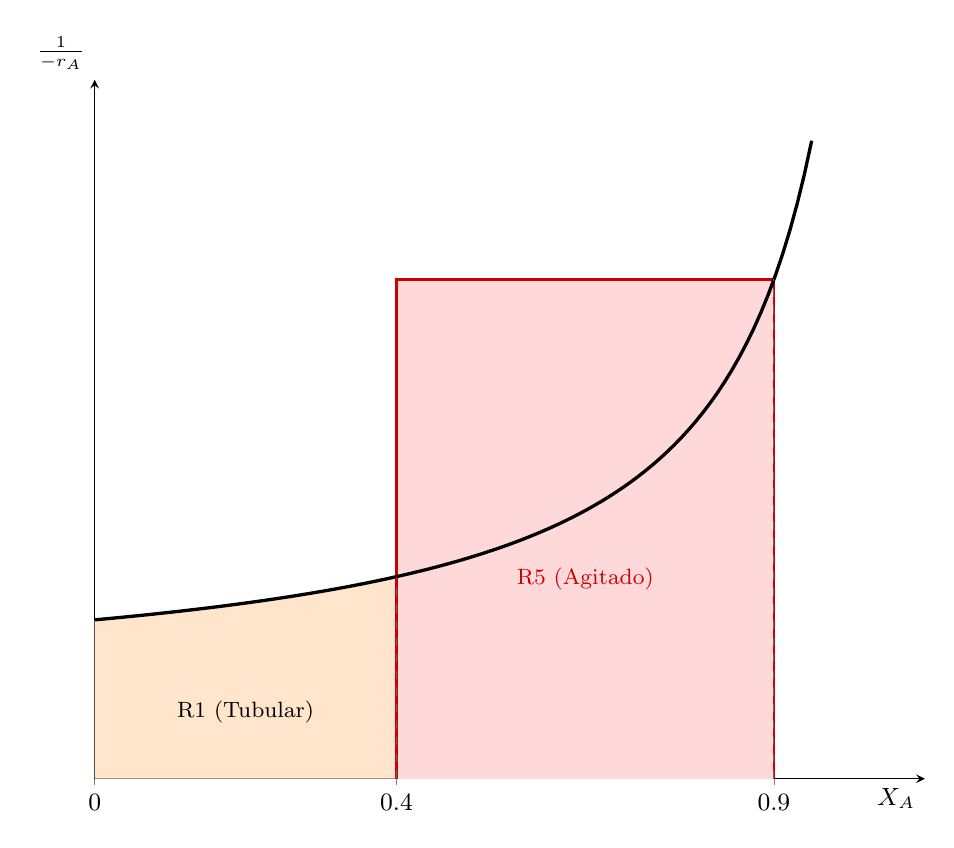
\begin{tikzpicture}
            \begin{axis}[
                    width=\linewidth,
                    axis lines=left,
                    xmin=0, xmax=1.1,
                    ymin=0, ymax=4.2,
                    xlabel={$X_A$},
                    ylabel={$\frac{1}{-r_A}$},
                    xlabel style={at={(ticklabel* cs:1)}, anchor=north east},
                    ylabel style={at={(ticklabel* cs:1)}, anchor=south east, rotate=270},
                    xtick={0, 0.4, 0.9},
                    xticklabels={0, $0.4$, $0.9$},
                    ytick=\empty,
                    label style={font=\small},
                    tick label style={font=\small},
                    domain=0:0.95,
                    samples=100
                ]
                % Área 1: Tubular (PFR) - Área bajo la curva de 0 a 0.4 (Naranja)
                \addplot [fill=orange!20, draw=none, domain=0:0.4] {0.5 + 0.5/(1.1-x)} \closedcycle;

                % Área 2: Tanque Agitado (CSTR) - Rectángulo de 0.4 a 0.9 con altura f(0.9) (Rojo coral)
                % f(0.9) = 3.0
                \fill [red!15] (axis cs:0.4,0) rectangle (axis cs:0.9,3.0);
                \draw [red!80!black, thick] (axis cs:0.4,0) -- (axis cs:0.4,3.0) -- (axis cs:0.9,3.0) -- (axis cs:0.9,0);

                % Curva 1/(-r_A)
                \addplot [very thick, black, domain=0:0.95] {0.5 + 0.5/(1.1-x)};

                % Líneas discontinuas de referencia
                \draw [dashed, black!60] (axis cs:0.4,0) -- (axis cs:0.4,1.214);
                \draw [dashed, black!60] (axis cs:0.9,0) -- (axis cs:0.9,3.0);

                % Etiquetas de volumen
                \node at (axis cs:0.2, 0.4) [anchor=center, font=\footnotesize] {R1 (Tubular)};
                \node at (axis cs:0.65, 1.2) [anchor=center, font=\footnotesize, color=red!80!black] {R5 (Agitado)};
            \end{axis}
        \end{tikzpicture}
        \caption{Tubular (hasta 40\%) + Agitado (hasta 90\%)}
        \label{fig:levenspiel_a}
    \end{subfigure}
    \hfill
    % Subfigura 2: Tanque Agitado (0 a 40%) + Reactor Tubular (40% a 90%)
    \begin{subfigure}[b]{0.48\textwidth}
        \centering
        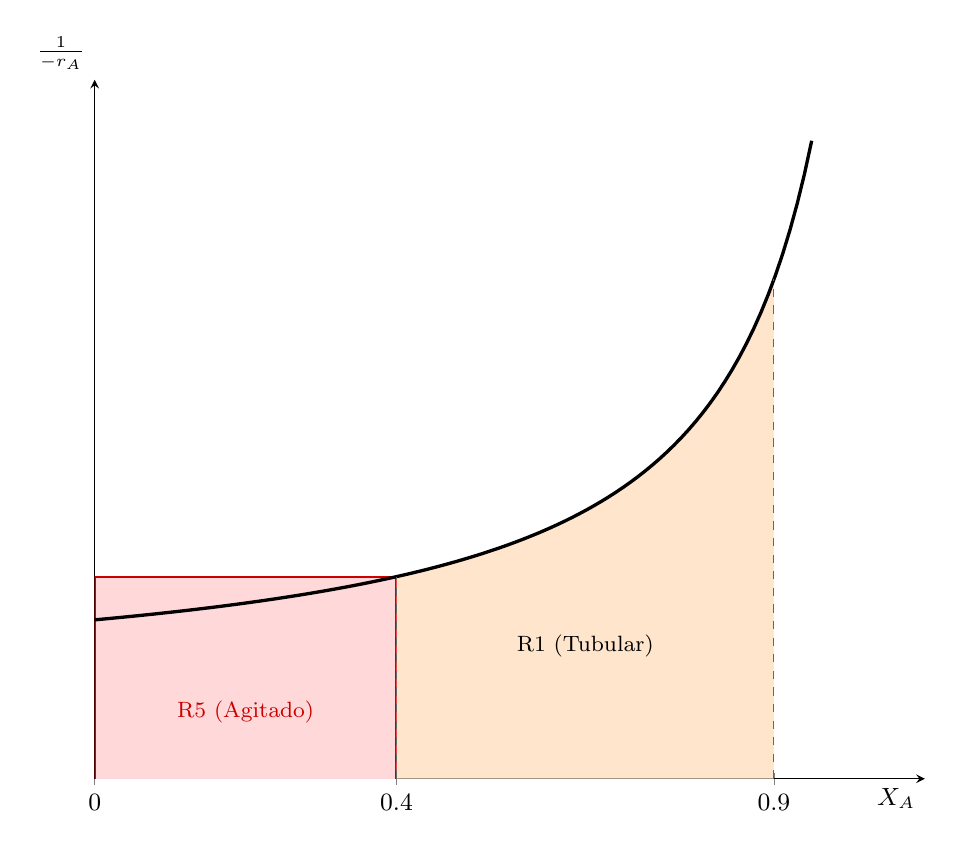
\begin{tikzpicture}
            \begin{axis}[
                    width=\linewidth,
                    axis lines=left,
                    xmin=0, xmax=1.1,
                    ymin=0, ymax=4.2,
                    xlabel={$X_A$},
                    ylabel={$\frac{1}{-r_A}$},
                    xlabel style={at={(ticklabel* cs:1)}, anchor=north east},
                    ylabel style={at={(ticklabel* cs:1)}, anchor=south east, rotate=270},
                    xtick={0, 0.4, 0.9},
                    xticklabels={0, $0.4$, $0.9$},
                    ytick=\empty,
                    label style={font=\small},
                    tick label style={font=\small},
                    domain=0:0.95,
                    samples=100
                ]
                % Área 1: Tanque Agitado (CSTR) - Rectángulo de 0 a 0.4 con altura f(0.4) (Rojo coral)
                % f(0.4) = 1.214
                \fill [red!15] (axis cs:0,0) rectangle (axis cs:0.4,1.214);
                \draw [red!80!black, thick] (axis cs:0,0) -- (axis cs:0,1.214) -- (axis cs:0.4,1.214) -- (axis cs:0.4,0);

                % Área 2: Tubular (PFR) - Área bajo la curva de 0.4 a 0.9 (Naranja)
                \addplot [fill=orange!20, draw=none, domain=0.4:0.9] {0.5 + 0.5/(1.1-x)} \closedcycle;

                % Curva 1/(-r_A)
                \addplot [very thick, black, domain=0:0.95] {0.5 + 0.5/(1.1-x)};

                % Líneas discontinuas de referencia
                \draw [dashed, black!60] (axis cs:0.4,0) -- (axis cs:0.4,1.214);
                \draw [dashed, black!60] (axis cs:0.9,0) -- (axis cs:0.9,3.0);

                % Etiquetas de volumen
                \node at (axis cs:0.2, 0.4) [anchor=center, font=\footnotesize, color=red!80!black] {R5 (Agitado)};
                \node at (axis cs:0.65, 0.8) [anchor=center, font=\footnotesize] {R1 (Tubular)};
            \end{axis}
        \end{tikzpicture}
        \caption{Agitado (hasta 40\%) + Tubular (hasta 90\%)}
        \label{fig:levenspiel_b}
    \end{subfigure}
    \caption{Comparación de configuraciones en serie de reactores R1 (Tubular) y R5 (Tanque agitado).}
    \label{fig:levenspiel_serie}
\end{figure}
\noindent Donde claramente se ve que seria mas eficiente el caso B es decir poner el reactor 5 primero y despues el 1 ya que ocuparian un menor volumen que seria la sumatoria de las areas representadas en cada caso siendo la naranja para el tubular y la roja para el agitado.
\newpage
\section{Examen junio 2020}

\qs{Ejercicio 1 (1 punto)}{
    En una planta se dispone de tres reactores de 1000 litros. Para su caracterización se realizan estudios del grado de mezcla mediante experimentos estímulo-respuesta en impulso.

    \textbf{Reactor 1:}
    \begin{center}
        \begin{tabular}{|c|c|c|c|c|c|c|c|c|c|c|c|}
            \hline
            $\theta$     & 0 & 0.2   & 0.4   & 0.6   & 0.8   & 1     & 1.5   & 2     & 3     & 5     & 8 \\ \hline
            $C_B/C_{BR}$ & 1 & 0.819 & 0.670 & 0.549 & 0.449 & 0.368 & 0.223 & 0.135 & 0.050 & 0.007 & 0 \\ \hline
        \end{tabular}
    \end{center}

    \textbf{Reactor 2:}
    \begin{center}
        \begin{tabular}{|c|c|c|c|c|c|c|c|c|c|c|c|}
            \hline
            $\theta$     & 0 & 0.25 & 0.50 & 0.75 & 1    & 1.5  & 2    & 2.5 & 3    & 4    & 5 \\ \hline
            $C_B/C_{BR}$ & 1 & 0.48 & 0.29 & 0.26 & 0.18 & 0.15 & 0.12 & 0.1 & 0.08 & 0.05 & 0 \\ \hline
        \end{tabular}
    \end{center}

    \textbf{Reactor 3:}
    \begin{center}
        \begin{tabular}{|c|c|c|c|c|c|c|c|c|c|c|c|c|}
            \hline
            $\theta$     & 0 & 0.25 & 0.50 & 0.75 & 1    & 1.25 & 1.5 & 2    & 2.5 & 3    & 3.5  & 4 \\ \hline
            $C_B/C_{BR}$ & 0 & 0.35 & 0.6  & 0.82 & 0.95 & 0.3  & 0.2 & 0.15 & 0.1 & 0.05 & 0.02 & 0 \\ \hline
        \end{tabular}
    \end{center}

    Con los datos obtenidos justifica el tipo de reactor y modelización.
}

\qs{Ejercicio 2 (1.5 puntos)}{
    En la planta se quiere llevar a cabo la reacción exotérmica de primer orden $A \rightarrow P$, a $T = 350 \text{ K}$. A esa temperatura la constante cinética es $0.3 \text{min}^{-1}$. Para un caudal de alimentación $F = 5X \text{ litros/min}$, donde $X$ es el primer número de tu DNI, justifica, mediante el cálculo correspondiente de la conversión de salida, el reactor que emplearías de los tres anteriores. En el caso en qué puedas justificar más de una forma de modelización para un reactor, aplícalas todas y calcula la conversión de salida en cada una de ellas.
}

\qs{Ejercicio 3 (1.5 puntos)}{
    Para el siguiente proceso de reacción en serie-paralelo:
    \begin{center}
        \begin{tabular}{lll}
            $A + B \rightarrow P$ ($P$ es el producto deseado) & $E_{a1} > E_{a2}$ & $r_1 = k_1 C_A C_B$   \\
            $P + 2B \rightarrow Q$ (reacción secundaria)       &                   & $r_2 = k_2 C_P C_B^2$
        \end{tabular}
    \end{center}

    \begin{enumerate}[label={\alph*)}]
        \item Justifica el tipo de reactor y condiciones de proceso donde lo llevaría a cabo para maximizar selectividad.
        \item Modeliza el funcionamiento del reactor mediante los balances que permitan determinar la evolución de la concentración de cada uno de los componentes.
        \item ¿Podrías mejorar aún más la selectividad del proceso actuando sobre el reactor elegido? ¿Se te ocurre alguna forma?
    \end{enumerate}
}
\newpage
\section{2023}

\shorthandoff{>}
\shorthandoff{<}

\qs{Ejercicio 1 (1 punto)}{
    Asocia a cada uno de los siguientes sistemas de reacción elementales, justifica la configuración y modo de operación del reactor, considerando como objetivo minimizar el volumen de reacción o maximizar la concentración del producto de interés (estos sistemas son operativos en el rango de temperaturas entre $T_{min}$ y $T_{max}$):

    \begin{enumerate}[label=\Roman*.]
        \item $A_{(g)} + B_{(g)} \rightarrow P_{(g)}$
        \item $2A_{(l)} + \text{catalizador}_{(s)} \rightarrow P_{(l)}$
        \item $2A_{(l)} + B_{(l)} \rightarrow P_{(l)}$ (producto deseado) \quad $E_{a1} < E_{a2}$ \\
              $A_{(l)} + 2B_{(l)} \rightarrow Q_{(l)}$ (reacción secundaria)
        \item $A_{(l)} + B_{(l)} \rightarrow P_{(l)}$ (producto deseado) \quad $E_{a1} > E_{a2}$ \\
              $2A_{(l)} + B_{(l)} \rightarrow Q_{(l)}$ (reacción secundaria)
        \item $A_{(l)} \rightleftharpoons B_{(l)}$ \quad proceso exotérmico
        \item $A_{(l)} + B_{(g)} \rightarrow P_{(l)}$
    \end{enumerate}
}

\tikzset{>=stealth}
\qs{Ejercicio 2 (1.5 puntos)}{
    Se dispone de dos reactores tipo tanque agitado, cuyos volúmenes son $V_1=V$ y $V_2=2V$ para llevar a cabo a temperatura constante, una reacción irreversible $A \rightarrow P$ de primer orden. Para un caudal de alimentación $F$, ¿Cuál de las siguientes ordenaciones daría una mayor producción de P? Puede suponerse que $k \cdot V/F = 1$

    \begin{enumerate}[label={\alph*)}]
        \item
              \begin{center}
                  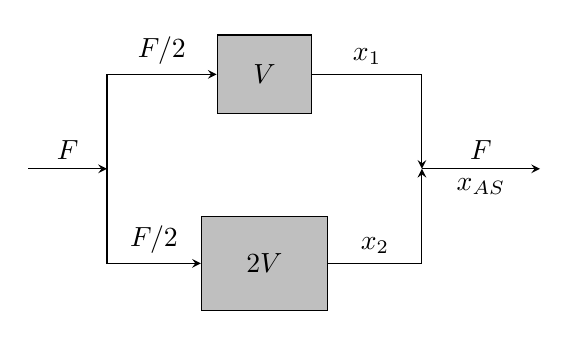
\begin{tikzpicture}[auto]
                      \coordinate (start) at (0,0);
                      \coordinate (split) at (1,0);
                      \node[draw, minimum width=1.2cm, minimum height=1cm, fill=lightgray] (V) at (3,1.2) {$V$};
                      \node[draw, minimum width=1.6cm, minimum height=1.2cm, fill=lightgray] (2V) at (3,-1.2) {$2V$};
                      \coordinate (join) at (5,0);
                      \coordinate (end) at (6.5,0);

                      \draw[->] (start) -- (split) node[midway,above] {$F$};
                      \draw[->] (split) -- (1,1.2) -- (V) node[midway,above] {$F/2$};
                      \draw[->] (split) -- (1,-1.2) -- (2V) node[midway,above] {$F/2$};
                      \draw[->] (V) -- (5,1.2) node[midway,above] {$x_1$} -- (join);
                      \draw[->] (2V) -- (5,-1.2) node[midway,above] {$x_2$} -- (join);
                      \draw[->] (join) -- (end) node[midway,above] {$F$} node[midway,below] {$x_{AS}$};
                  \end{tikzpicture}
              \end{center}
        \item
              \begin{center}
                  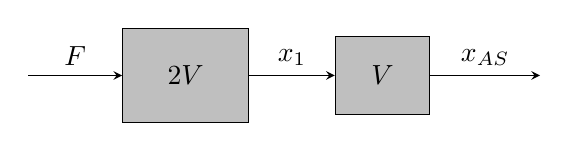
\begin{tikzpicture}[auto]
                      \coordinate (start) at (0,0);
                      \node[draw, minimum width=1.6cm, minimum height=1.2cm, fill=lightgray] (2V) at (2,0) {$2V$};
                      \node[draw, minimum width=1.2cm, minimum height=1cm, fill=lightgray] (V) at (4.5,0) {$V$};
                      \coordinate (end) at (6.5,0);

                      \draw[->] (start) -- (2V) node[midway,above] {$F$};
                      \draw[->] (2V) -- (V) node[midway,above] {$x_1$};
                      \draw[->] (V) -- (end) node[midway,above] {$x_{AS}$};
                  \end{tikzpicture}
              \end{center}
        \item
              \begin{center}
                  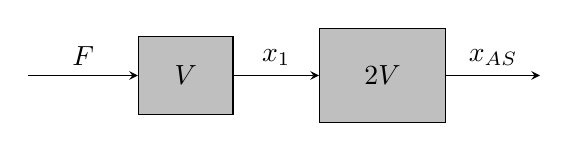
\begin{tikzpicture}[auto]
                      \coordinate (start) at (0,0);
                      \node[draw, minimum width=1.2cm, minimum height=1cm, fill=lightgray] (V) at (2,0) {$V$};
                      \node[draw, minimum width=1.6cm, minimum height=1.2cm, fill=lightgray] (2V) at (4.5,0) {$2V$};
                      \coordinate (end) at (6.5,0);

                      \draw[->] (start) -- (V) node[midway,above] {$F$};
                      \draw[->] (V) -- (2V) node[midway,above] {$x_1$};
                      \draw[->] (2V) -- (end) node[midway,above] {$x_{AS}$};
                  \end{tikzpicture}
              \end{center}
    \end{enumerate}
}

\qs{Ejercicio 3 (1.5 puntos)}{
    En una planta química se construyó un RCMP para llevar a cabo una reacción irreversible de primer orden y conseguir un 75\% de conversión ($\tau \cdot k = 3$). Sin embargo, en la puesta en marcha se comprueba que la conversión final obtenida es ligeramente menor que la descrita por el modelo ideal. Entonces, se le realizan estudios del grado de mezcla mediante experimentación estímulo-respuesta en impulso. Se obtienen los siguientes datos:

    \begin{center}
        \begin{tabular}{|c|c|c|c|c|c|c|c|c|c|c|c|c|c|c|}
            \hline
            $t$, min   & 0 & 1 & 2    & 3    & 4    & 5    & 6    & 7    & 8    & 9    & 10   & 11   & 12   & 13 \\ \hline
            $c_s$, g/L & 0 & 0 & 0.02 & 0.35 & 0.88 & 1.01 & 0.78 & 0.47 & 0.24 & 0.12 & 0.05 & 0.02 & 0.01 & 0  \\ \hline
        \end{tabular}
    \end{center}

    \begin{enumerate}[label={\alph*)}]
        \item Justifica el comportamiento del reactor y discute la modelización más adecuada.
        \item ¿Es aplicable el modelo de flujo segregado?
        \item Calcula la conversión real del reactor.
    \end{enumerate}
}

% \shorthandon{>}
% \shorthandon{<}
\newpage
\section{2024}

\qs{Ejercicio 1}{
    En una planta química se produce P por transformación de A: $A \rightarrow P$. $r_1 = k_1 C_A$.
    En las condiciones de reacción tiene lugar la formación de un dímero de A que da
    lugar a Q, producto no deseado, $2A \rightarrow Q$ ; $r_2 = k_2 C_A^2$.
    Al ser una cinética potencial el proceso se estaba llevando a cabo en un reactor
    tubular. El nuevo becario defiende que se pueden obtener mejores resultados si el
    proceso se lleva a cabo en un reactor tanque agitado. ¿Cuál crees que es la mejor
    forma de llevar a cabo ese proceso?}
\begin{table}[h]
    \centering
    \caption{Valores adimensionales de los experimentos RTD ($\tau = 10$ min)}
    \label{tab:integrales_adimensionales}
    \begin{tabular}{lccc}
        \toprule
        \textbf{Reactor} & \textbf{$\int E \, d\theta$} & \textbf{$\int \theta E \, d\theta$} & \textbf{$\int \theta^2 E \, d\theta$} \\ \midrule
        Reactor 1        & 1.00                         & 0.99                                & 1.07                                  \\
        Reactor 2        & 1.00                         & 1.00                                & 1.95                                  \\
        Reactor 3        & 0.91                         & 0.85                                & 1.40                                  \\\bottomrule
    \end{tabular}
\end{table}
\nt{Las tablas no son las proporcionadas, pero los valores permiten contestar la pregunta.}
\qs{Ejercicio 2}{
    El reactor tubular de la planta se ha roto, por lo que en cualquier caso hay que
    cambiarlo. Se le encarga al becario que analice 3 reactores que hay en el
    almacén de volumen V (igual al reactor roto) y justifique cual es el reactor mas
    idóneo.
    El becario decide hacerles estudios fluidodinámicos por experimentos estimulo-
    respuesta en impulso
    \begin{enumerate}[label={\alph*)}]
        \item Analiza resultados obtenidos e indica configuración y modalización para el
              cálculo de $X_s$ en cada reactor
        \item Reactor que utilizarías para reemplazar el reactor tubular que se ha roto.

        \item Con el nuevo se obtendrá +P o -P, como crees que cambiaria la Concentración de P y $\tau$, y F y
              productividad.

        \item ¿Qué aconsejarías a la empresa para optimizar la productividad y
              selectividad?

    \end{enumerate}
}
\newpage
\section{??}
\qs{Ejercicio 1 (1.5 puntos)}{Para la reacción elemental irreversible exotérmica en fase líquida \textbf{$A \rightarrow P$}, deduce la expresión para calcular el tiempo de reacción o tiempo espacial si se desea conseguir una conversión $X_{AS}$ en un reactor isotérmico con un caudal $F$.
}
\solve{}
\begin{enumerate}[label={\alph*)}]
    \item Reactor continuo mezcla perfecta

          \noindent Modelizando:
          \begin{align*}
              \frac{dM}{dt}                     & = m_0 - m_s                                                                  \\[6pt]
              \sum m_0                          & = \sum m_s                                                                   \\[6pt]
              \frac{dN}{dt}                     & = n_0 - n_s + r_i \cdot V                                                    \\[6pt]
              \frac{d(C \cdot V)}{dt}           & = F(C_0 - C_s) + r_i \cdot V                                                 \\[6pt]
              \frac{d(M \cdot C_p \cdot T)}{dt} & = m \cdot C_p \cdot (T_0 - T) + V \sum_{k=1}^{h} \Delta H_k \cdot r_k + Q(T)
          \end{align*}
          \noindent Para la reacción que nos indican en el enunciado $A \rightarrow P$ exotérmica y en isotermo, partiendo de las ecuaciones generales anteriores:
          \begin{equation*}
              \frac{dN_A}{dt} = n_{A0} - n_{As} - r_A \cdot V
          \end{equation*}
          \noindent En el estado estacionario:

          \begin{equation*}
              \frac{dN_A}{dt} = 0
          \end{equation*}

          \begin{equation*}
              N_{AR}\cdot (1-X_{A0}) - N_{AR}(1-X_{AS}) - (r_A)_s \cdot V = 0
          \end{equation*}
          \vspace{1em}
          \noindent Recordando que $\tau$ se define como $\frac{V}{F}$.
          \begin{equation*}
              (r_A)_s \cdot V = N_{AR}\cdot (X_{AS}-X_{A0}) \implies \tau = \frac{C_{AR}\cdot (X_{AS}- X_{A0})}{(r_A)_s}
          \end{equation*}

          \noindent Si graficamos la temperatura respecto a la conversión de A, según la temperatura seleccionada siempre se llegará a la conversión deseada, pero a medida que se aumenta la temperatura se llega antes a ese punto; por tanto, la condición $T = \text{const}$ será $T = T_{\text{máx}}$.

          \begin{figure}[htbp]
              \centering
              \begin{tikzpicture}[
                      scale=1.1,
                      >=Latex,
                      font=\small
                  ]

                  % Ejes
                  \draw[thick,->] (0,0) -- (5.8,0) node[below] {$x_A$};
                  \draw[thick,->] (0,0) -- (0,4.5) node[left] {$T$};

                  % Punto común
                  \coordinate (Azeo) at (4.8,0);

                  % Curvas
                  \draw[thick]
                  (1.00,4.00)
                  .. controls (1.60,2.80) and (3.40,0.70)
                  .. (Azeo);

                  \draw[thick]
                  (1.55,4.00)
                  .. controls (2.10,2.90) and (3.80,0.90)
                  .. (Azeo);

                  \draw[thick]
                  (2.20,4.00)
                  .. controls (2.80,3.00) and (4.10,1.10)
                  .. (Azeo);

                  % Etiquetas de curvas
                  \node at (0.75,2.55) {$t_1$};
                  \node at (1.45,4.20) {$T_1$};
                  \node at (2.10,4.20) {$T_2$};
                  \node at (2.80,4.20) {$T_3$};

                  % Composición azeotrópica
                  \draw[densely dashed]
                  (Azeo) -- ++(0,0.45);

                  \node[below] at (Azeo) {$x_{A,S}$};

                  % Temperatura máxima
                  \node[right] at (5.15,2.8)
                  {$T = T_{\text{máx}}$};

              \end{tikzpicture}

              \caption{Temperatura vs Conversión en reacción irreversible exotérmica.}
              \label{fig:temp_max}
          \end{figure}
    \item Reactor flujo pistón
          \begin{align}
              \frac{dN_A}{dt}   & = n_A - (n_A + dn_A) - r_A \cdot dV \nonumber                               \\
              -dn_A             & = r_A \cdot dV \nonumber                                                    \\
              dn_A              & = n_{AR} \cdot dX_A \nonumber                                               \\
              n_{AR} \cdot dX_A & = r_A \cdot dV \nonumber                                                    \\
              \int_0^V dV       & = n_{AR} \int_{X_{A0}}^{X_{AR}} \frac{dX_A}{r_A} \nonumber                  \\
              V                 & = n_{AR} \int_{X_{A0}}^{X_{AS}} \frac{dX_A}{r_A} \nonumber                  \\
              \frac{V}{F}       & = \frac{n_{AR}}{F} \int_{X_{A0}}^{X_{AS}} \frac{dX_A}{r_A} \nonumber        \\
              \tau              & = C_{AR} \int_{X_{A0}}^{X_{AS}} \frac{dX_A}{r_A} \label{eq:RCFP_examen_unk}
          \end{align}
          \noindent La temperatura de reacción se justifica de forma análoga al caso anterior, siendo esta $T_{\text{máx}}$.
    \item Dos reactores mezcla perfecta en serie.

          \noindent En este caso se usan los mismos balances que en el caso anterior, pero definiendo el tiempo espacial para cada reactor como $\tau_i = V_i/F$. Es decir, cada reactor divide el volumen total entre el número de reactores.
          \begin{align*}
              \frac{\tau_i}{C_{AR}} & = \frac{X_{Ai}-X_{A(i-1)}}{-r_{Ai}}                                                                                              \\[6pt]
              \tau_i                & = \frac{C_A \cdot (X_{A1}-0)}{C_{A0}\cdot K \cdot (1-X_{A1})} = \frac{C_A \cdot (X_{AS}-X_{A1})}{C_{A0}\cdot K \cdot (1-X_{AS})} \\[6pt]
              \tau                  & = 2 \cdot \tau_i
          \end{align*}
          \noindent Como la reacción es la misma, la temperatura de operación óptima vuelve a ser $T_{\text{máx}}$.
          \newpage
    \item Reactor flujo pistón con recirculación.
          \begin{figure}[H]
              \centering
              
\includegraphics[width=0.75\textwidth]{PFR_recirculacion.png}
              \caption{Recirculación en el RCFP}
          \end{figure}
          \noindent Siendo $R$ la relación de caudal de recirculación entre el caudal de salida, es decir:

          \begin{equation*}
              R = \frac{\text{caudal de recirculación}}{\text{caudal de salida}} = \frac{F_R}{F}
          \end{equation*}

          \noindent El balance de materia en el punto de mezcla queda de la siguiente forma:
          \begin{align*}
              F \cdot C_{A0} + F_R \cdot C_{AS} & = F(1 + R)C_{Ae}                                                                            \\[6pt]
              C_{Ae}                            & = \frac{C_{A0} + R \cdot C_{AS}}{1 + R} \quad ; \quad X_{Ae} = \frac{C_{AR}-C_{Ae}}{C_{AR}} \\[6pt]
              X_{Ae}                            & = \frac{X_{A0} + R\cdot X_{AS}}{1+R}
          \end{align*}
          \noindent Introduciéndolo en la ecuación del flujo pistón~\eqref{eq:RCFP_examen_unk} obtenemos:
          \begin{equation*}
              \tau = (1+R)\cdot C_{AR}\int_{X_{Ae}}^{X_{AS}}-\frac{dX_A}{r_A}
          \end{equation*}
          \noindent Con $T$ constante a $T_{\text{máx}}$.
    \item Ordena de menor volumen a mayor volumen necesario los sistemas anteriores.
          \noindent La forma de justificarlo es mediante los gráficos de Levenspiel (ver figura~\ref{fig:levenspiel_a}). El reactor que mayor volumen ocupa siempre es el reactor continuo de mezcla perfecta (RCMP), y el reactor de flujo pistón (RCFP) es el que menos. Para los otros dos casos se sigue el siguiente razonamiento:
          Cuando se tiene un reactor de tanques en serie, se forman escalones en el gráfico de Levenspiel. Si $n \to \infty$, estaríamos en el caso límite de un flujo pistón. Al variar $n$, el comportamiento del sistema se desplaza desde un mezcla perfecta ($n=1$) hacia un flujo pistón.
          Para el caso del flujo pistón con recirculación ocurre algo similar según varíe la relación de recirculación: si $R \to 0$, es equivalente a un flujo pistón puro porque no existe recirculación. Por el contrario, si $R \to \infty$ (entendiendo infinito como un número lo suficientemente grande), todo se estaría recirculando, por lo que equivaldría a un reactor de mezcla perfecta. Así, el orden de menor a mayor volumen requerido es:
          \begin{center}
              \vspace{1em}
              \Res{\parbox{12cm}{\vspace{1em} \centering $\text{RCFP} < \underbrace{\text{RCFP}_{\text{recirculación}}}_{R \to 0} < 2\text{RCMP} < \underbrace{\text{RCFP}_{\text{recirculación}}}_{R \to \infty} < \text{RCMP}$}}
          \end{center}
\end{enumerate}
\newpage
\qs{Ejercicio 2}{En una planta química se dispone de tres unidades de reacción de $60\text{ m}^3$ cada una con un caudal de $200\ \text{L}/\text{min}$. Tras realizar un experimento de estímulo-respuesta en impulso en cada una de ellas, se obtienen los valores de las integrales de distribución de tiempo de residencia (RTD) mostrados en la tabla adjunta. Justifica el comportamiento real de cada reactor e indica el modelo más adecuado a emplear. ¿Cuál de ellos seleccionarías para llevar a cabo una reacción de primer orden? Calcula la conversión de salida para el modelo de reactor que elijas.}

\begin{table}[htbp]
    \centering
    \caption{Valores adimensionales de las integrales RTD para los reactores R1, R2 y R3.}
    \label{tab:integrales_ejercicio2}
    \begin{tabular}{cccc}
        \toprule
        \textbf{Reactor} & \textbf{$\int E \, d\theta$} & \textbf{$\int \theta E \, d\theta$} & \textbf{$\int \theta^2 E \, d\theta$} \\ \midrule
        R1               & $1$                          & $1$                                 & $4/3$                                 \\
        R2               & $0.85$                       & $0.70$                              & --                                    \\
        R3               & $1$                          & $1$                                 & $1.75$                                \\ \bottomrule
    \end{tabular}
\end{table}
\solve{}
\begin{enumerate}[label={\alph*)}]
    \item Justifica el comportamiento real de cada reactor e indica el modelo más adecuado a emplear.
          \begin{itemize}
              \item \textbf{Para el reactor 1:}
                    No existe bypass ni volumen estanco, ya que $\int E\,d\theta = 1$ y $\int \theta E\,d\theta = 1$. Con la última integral se calcula la varianza:
                    \begin{equation*}
                        \sigma^2 = \int \theta^2 E\,d\theta - 1 = 4/3 -1 = 1/3
                    \end{equation*}
                    Puesto que está más cerca de 0 que de 1, se asemeja más a un reactor continuo de flujo pistón. Es decir, estamos ante un reactor tubular debido a que no presenta un comportamiento ideal. Este se puede modelar con el modelo de flujo segregado (al ser de primer orden), el modelo de dispersión y el modelo de tanques en serie, el cual será el siguiente:
                    \begin{equation*}
                        \sigma^2 = \frac{1}{n} \implies n = 3
                    \end{equation*}
                    Con el flujo segregado, la modelización sería la siguiente:
                    \begin{equation*}
                        \overline{C_A} = \int_{0}^{\infty} C_A(\theta) \cdot E \, d\theta
                    \end{equation*}
                    En función de la conversión, sería:
                    \begin{equation*}
                        1 -\overline{X_A} = \int_{0}^{\infty} 1 - X_A(\theta) \cdot E \, d\theta
                    \end{equation*}
                    \begin{align*}
                        \left.\begin{aligned}
                                  \frac{dC_A}{dt} & = r_A     \\
                                  r_A             & = -k\,C_A
                              \end{aligned}\right\}
                        \implies \frac{dC_A}{dt} = -k\,C_A
                        \implies \cancel{C_{A0}}\frac{dX_A}{dt} = -k\,\cancel{C_{A0}}(1-X_A)
                    \end{align*}
                    \begin{align*}
                         & \frac{dX_A}{dt}                       = -k(1-X_A)\quad \frac{dX_A}{1-X_A} = -k dt  \\[6pt]
                         & \int_{0}^{X_{AS}} \frac{dX_A}{1-X_A}  = -k \int_{0}^{t} dt                         \\[6pt]
                         & -ln(1-X_{AS})                         = -kt \implies 1-X_A = \text{exp}(-k\cdot t)
                    \end{align*}
                    Expresándolo en función del tiempo de residencia, es decir, $t = t_R \cdot \theta$:
                    \begin{equation*}
                        \boxed{1-X_A(\theta) = \text{exp}(-k\cdot t_R \cdot \theta)}
                    \end{equation*}
                    \nt{Esta modelización se podría aplicar en los tres reactores, puesto que solo depende de que la reacción sea de primer orden.}

              \item \textbf{Para el reactor 2:}

                    \noindent Solo existe una opción de modelización: la de modelos mezclados. El reactor es de tipo tanque agitado.
              \item \textbf{Para el reactor 3:}\\
                    No existe bypass ni volumen estanco, puesto que $\int E\,d\theta = 1$ y $\int \theta E\,d\theta = 1$. Con la última integral se calcula la varianza:
                    \begin{equation*}
                        \sigma^2 = \int \theta^2 E\,d\theta - 1 = 1.75 -1 = 0.75
                    \end{equation*}
                    Por lo tanto, estamos ante un reactor de tipo tanque agitado, el cual modelizamos como un RCFP con recirculación (RCFP-R), recordando que la recirculación se puede calcular mediante la varianza:
                    \begin{equation*}
                        \sigma^2 = \frac{1}{1+R} \quad \implies R = 3
                    \end{equation*}
          \end{itemize}
    \item ¿Cuál utilizarías para llevar a cabo la reacción en fase líquida $A \rightarrow P$ de primer orden?\\
          Se puede elegir tanto el reactor 1 como el 3. Lo correcto es calcular la conversión de ambos y elegir el que dé mayor conversión. Sin embargo, en este caso, al tratarse de una reacción irreversible de primer orden, conviene elegir uno que funcione con perfil de concentraciones; es decir, o bien un reactor tubular (si su comportamiento es de flujo pistón ideal) o bien un tanque agitado en modo de operación discontinua.
          \begin{itemize}
              \item Reactor 1
                    \begin{equation*}
                        \tau_{i} = \frac{\tau}{n} = \frac{300}{3} = 100\text{min}
                    \end{equation*}
                    \begin{equation*}
                        100 = \frac{X_{A1}-0}{0.01(1-X_{A1})} = \frac{X_{A2}-X_{A1}}{0.01(1-X_{A2})} = \frac{X_{AS}-X_{A2}}{0.01(1-X_{AS})} \implies X_{AS} = 0.875
                    \end{equation*}
                    \nt{$X_{A1} = 0.5$ , $X_{A2} = 0.75$ y $X_{AS} = 0.875$}
              \item Reactor 3
                    \begin{equation*}
                        \frac{60\text{m}^3}{0.2\text{m}^3/\text{min}} = (1+3)\cdot \cancel{C_{AR}}\int_{X_{\dfrac{X_{AS}\cdot R}{1+R}}}^{X_{AS}}-\frac{dX_A}{k\cdot \cancel{C_{AR}}\cdot (1-X_A)} \implies X_{AS} = 0.817
                    \end{equation*}
          \end{itemize}
    \item Calcula la conversión de salida con el reactor que has elegido.\\
          \noindent Se ha realizado en el apartado anterior.
          \begin{center}
              \vspace{1em}
              \Res{\text{El reactor elegido es el 1, ya que se logra una mayor conversión de salida} \quad (0.875 > 0.817)}
          \end{center}
\end{enumerate}
\newpage
\qs{Ejercicio 3}{A) En un sistema de reacciones múltiples, define selectividad instantánea y selectividad global B) Determina su relación para un reactor continuo de mezcla perfecta y un flujo pistón}
\solve{}
\begin{enumerate}[label={\alph*)}]
    \item Selectividad instantánea y global:
          \begin{equation*}
              \text{Selectividad local} = \frac{\text{Velocidad de transformancion de A en P}}{\text{Velocidad de transformancion de A}}
          \end{equation*}
          Estando en estado estacionario para $A +B +\dots\rightarrow C +D +\dots \alpha P$ , para una reacción simple $A \rightarrow P$
          \nt{siendo $\alpha$ el coeficiente estequiometrico}
          \begin{equation*}
              S_p = \frac{\dfrac{r_P}{\alpha P}}{r_A}
          \end{equation*}
          Para evitar trabajar con velocidades y asi trabajar directamente con los moles , se usa la selectividad global es decir:
          \begin{equation*}
              S_G = \frac{\text{moles de A transformados en P}}{\text{moles de A transformados}}
          \end{equation*}

    \item Relación con RCFP Y RCMP
          \begin{itemize}
              \item RCFP: \\
                    Partiendo del balance:
                    \begin{equation*}
                        \frac{dNa}{dt} = n_A-(n_A+dn_A) + r_A \cdot dV
                    \end{equation*}
                    En estado estacionario:
                    \begin{align*}
                        -dn_A & = r_A \cdot dV \\
                        dn_P  & = r_P \cdot dV
                    \end{align*}
                    dividiendo ambas:
                    \begin{equation*}
                        \frac{dn_A}{dn_P} = \frac{r_A}{-r_P} \quad \, \quad S_G = \frac{1}{n_{A0}-n_{Af}}\int_{n_{Af}}^{n_{A0}} s \cdot dn_A
                    \end{equation*}
                    si la densidad es constante $\rho = \text{cte}$, entonces:
                    \begin{equation*}
                        S_G = \frac{1}{C_{A0}-C_{Af}}\int_{C_{Af}}^{C_{A0}} s \cdot dC_A
                    \end{equation*}

              \item Para el RCMP:
                    \begin{equation*}
                        \frac{dN_A}{dt} = n_{A0} - n_{Af} - r_A \cdot V
                    \end{equation*}
                    \begin{align*}
                        n_{A0} - n_{Af} & = (r_A)_f \cdot V  \\
                        n_{P0} - n_{Pf} & = -(r_P)_f \cdot V
                    \end{align*}

                    \begin{equation*}
                        \boxed{S_G = \frac{\dfrac{(n_{P0}-n_{Pf})}{\alpha P}}{(n_{A0}-n_{Af})} = \frac{\dfrac{-(r_{P})_f}{\alpha_P}}{-(r_{A})_f} = s_f}
                    \end{equation*}

          \end{itemize}
          \nt{Para los reactores Tubulares (flujo pistón en caso de ser ideales) la selectividad varia a lo largo de la reacción, mientras que en el reactor tipo tanque agitado la selectividad global es la selectividad final del reactor}
          \cor{En el caso de reacciones multiples}{
              \begin{itemize}
                  \item Reacciones paralelas:
                        \begin{align*}
                            A \rightarrow P \quad \, \quad r_1  & = k_1 \cdot C_A   \\
                            2A \rightarrow Q \quad \, \quad r_2 & = k_2 \cdot C_A^2
                        \end{align*}



                        Es decir $n_1 < n_2$
                        \begin{itemize}
                            \item Para el RCFP:
                                  \begin{align*}
                                      S_G = \frac{1}{C_{A0}-C_{Af}}\int_{C_{Af}}^{C_{A0}} \underbrace{s}_{\frac{r_1}{r_1+r_2}} \cdot dC_A
                                  \end{align*}
                                  \begin{align*}
                                      S_G & = \frac{1}{C_{A0}-C_{Af}}\int_{C_{Af}}^{C_{A0}}\frac{1}{1+\dfrac{k_2}{k_1}\cdot C_A} \cdot dC_A                                                          \\[6pt]
                                      S_G & = \frac{k_1}{k_2 \cdot C_{A0} \cdot X_{Af}}\cdot \ln \left( \frac{1+\dfrac{k_2}{k_1}\cdot C_{A0}}{1+\dfrac{k_2}{k_1}\cdot C_{A0}\cdot (1-X_{Af}} \right)
                                  \end{align*}
                            \item Para el RCMP:
                                  \begin{align*}
                                      S_G = \frac{1}{1+\dfrac{k_2}{k_1}\cdot C_{A0}\cdot (1-X_{Af})}
                                  \end{align*}
                        \end{itemize}
                  \item Reacciones paralelas:
                        \begin{align*}
                            2A \rightarrow P \quad \, \quad r_1 & = k_1 \cdot C_A^2 \\
                            A \rightarrow Q \quad \, \quad r_2  & = k_2 \cdot C_A
                        \end{align*}
                        Es decir $n_1 > n_2$.
                        \begin{itemize}
                            \item Para el RCFP:
                                  \begin{align*}
                                      S_G = \frac{1}{C_{A0}-C_{Af}}\int_{C_{Af}}^{C_{A0}} s \cdot dC_A
                                  \end{align*}
                                  \begin{align*}
                                      S_G & = \frac{1}{C_{A0}-C_{Af}}\int_{C_{Af}}^{C_{A0}}\frac{1}{1+\dfrac{k_2}{k_1}\cdot C_A} \cdot dC_A                            \\[6pt]
                                      S_G & = 1- \frac{k_2}{k_1\cdot C_{A0}\cdot X_{Af}} \cdot \ln \left( \frac{1}{1-\dfrac{k_2}{k_1}\cdot C_{A0}\cdot X_{Af}} \right)
                                  \end{align*}
                            \item Para el RCMP:
                                  \begin{align*}
                                      S_G = \frac{1}{1+\dfrac{k_2}{k_1}\cdot C_{A0}\cdot(1- X_{Af})}
                                  \end{align*}
                        \end{itemize}

              \end{itemize}
          }
          \begin{figure}[H]
              \centering
              \begin{subfigure}[b]{0.48\textwidth}
                  \centering
                  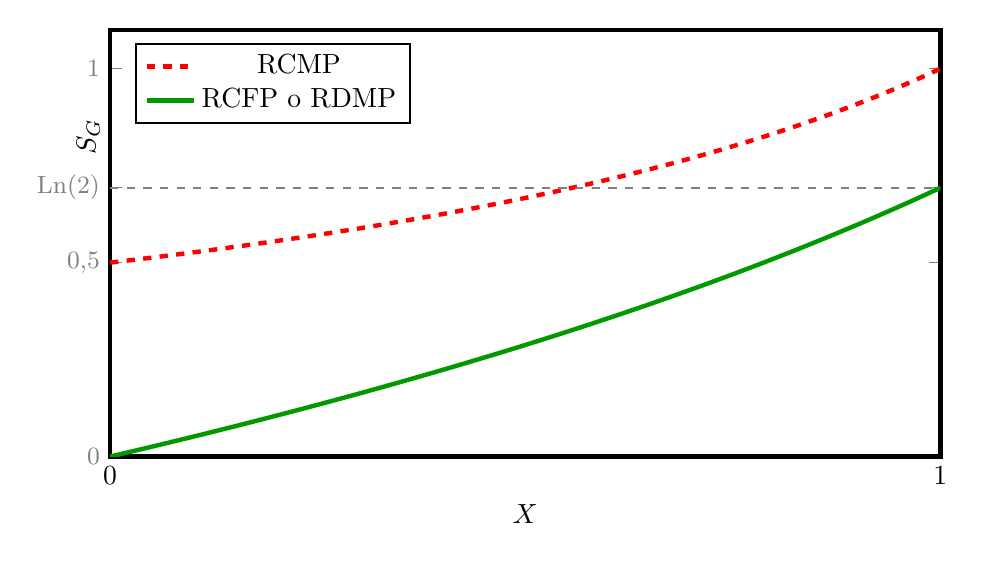
\begin{tikzpicture}
                      \begin{axis}[
                              width=\linewidth, height=7cm,
                              xmin=0, xmax=1, ymin=0, ymax=1.1,
                              xlabel={$X$}, ylabel={$S_G$},
                              ylabel style={
                                      at={(axis description cs:0, 0.75)},
                                      anchor=south,
                                      rotate=0
                                  },
                              yticklabel style={font=\small, color=gray},
                              axis line style={ultra thick},
                              ytick={0, 0.5, 0.693, 1},
                              yticklabels={0, {0,5}, {Ln(2)}, 1},
                              xtick={0, 1},
                              thick,
                              legend pos=north west
                          ]
                          % Curva Roja (RCMP): s_f = 1 / (2-X)
                          \addplot[red, ultra thick, dashed, domain=0:1, samples=100] {1 / (2 - x)};
                          \addlegendentry{RCMP}

                          % Curva Verde (RCFP): ln( 2 / (2-X) ) -> Esto es lo que dibujó ella
                          \addplot[green!60!black, ultra thick, domain=0:1, samples=100] {ln( 2 / (2 - x) )};
                          \addlegendentry{RCFP o RDMP}

                          % Línea guía Ln(2)
                          \draw[gray, dashed] (axis cs: 0, 0.693) -- (axis cs: 1, 0.693);
                      \end{axis}
                  \end{tikzpicture}
                  \caption{Selectividad global vs Conversión para el caso $n_1 < n_2$}
              \end{subfigure}
              \hfill
              \begin{subfigure}[b]{0.48\textwidth}
                  \centering
                  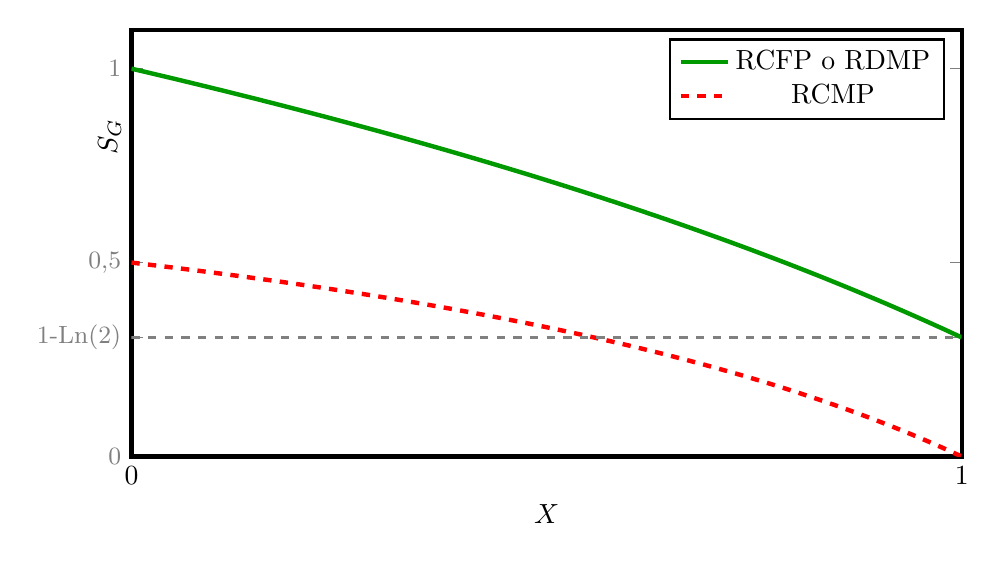
\begin{tikzpicture}
                      \begin{axis}[
                              width=\linewidth, height=7cm,
                              xmin=0, xmax=1, ymin=0, ymax=1.1,
                              xlabel={$X$}, ylabel={$S_G$},
                              ylabel style={
                                      at={(axis description cs:0, 0.75)},
                                      anchor=south,
                                      rotate=0
                                  },
                              yticklabel style={font=\small, color=gray},
                              axis line style={ultra thick},
                              ytick={0, 0.307, 0.5,1},
                              yticklabels={0, {1-Ln(2)}, {0,5}, 1},
                              xtick={0, 1},
                              thick,
                              legend style={anchor=north east}
                          ]
                          % Curva Verde (RCFP): 1 - (1/x)*ln(2/(2-x))
                          % Representa la selectividad global analítica para k1=k2=Ca0=1
                          \addplot[green!60!black, ultra thick, domain=0:1, samples=100] {1 - ln( 2 / (2-x) )};
                          \addlegendentry{RCFP o RDMP}

                          % Curva Roja (RCMP): (1-x)/(2-x)
                          \addplot[red, ultra thick, dashed, domain=0:1, samples=100] {(1-x)/(2-x)};
                          \addlegendentry{RCMP}

                          % Línea guía asintótica 1-Ln(2)
                          \draw[gray, dashed] (axis cs: 0, 0.307) -- (axis cs: 1, 0.307);
                      \end{axis}
                  \end{tikzpicture}
                  \caption{Comparativa de selectividad para $n_1 > n_2$}
              \end{subfigure}
              \caption{Selectividad global en función de la conversión para distintas cinéticas}
          \end{figure}
    \item Para el caso de reacciones en sistema en paralelo, ¿en qué reactor continuo llevarías a cabo la reacción? Justifica la respuesta.

          Se ha justificado en el apartado anterior, aunque tambien se puede justificar de la siguiente forma:
          \begin{itemize}
              \item Primer caso $n_2 > n_1$:
                    \begin{equation*}
                        s = \frac{r_1}{r_1+r_2} =  \frac{1}{1+\dfrac{r_2}{r_1}} = \frac{1}{1+\dfrac{k_2}{k_1}\cdot \dfrac{C_A^{\cancel{2}}}{\cancel{C_A}}}
                    \end{equation*}
                    es decir la concentración de A debe ser lo menor posible $C_A \downarrow$ y por tanto es el caso de un reactor continuo mezcla perfecta (RCMP).
              \item Segundo caso $n_1 > n_2$:
                    \begin{equation*}
                        s = \frac{r_1}{r_1+r_2} =  \frac{1}{1+\dfrac{r_2}{r_1}} = \frac{1}{1+\dfrac{k_2}{k_1}\cdot \dfrac{\cancel{C_A}}{C_A^{\cancel{2}}}}
                    \end{equation*}
                    es decir la concentración de A debe ser lo mayor posible $C_A \uparrow$ y por tanto es el caso de un flujo pistón (RCFP).
          \end{itemize}
\end{enumerate}